\section{引言}
无人机已经成为商业、工业、娱乐和执法的重要支援设备~\cite{chabot2018trends,banos2020assessment,patino2009adaptive,shukla2016application,huang2021multi,li2018uav}。
随着无人机越来越多地被用于关键任务,客户对无人机飞行的可靠性和稳定性有很高要求。
因此,无人机的软件开发者建立了一种安全检查系统来检测和缓解此类飞行过程中的安全问题。
这样的系统通常有不同的模块来处理不同的安全问题,如无人机坠毁、电机推力损失、角位置不平衡等。
模块通过应用它们的条件规则来检验特定的内部监测值(如特定角度)来判断相应的安全问题是否发生。
当检测到问题时,系统提供补救措施,例如,在检测到推力损失时启动动力助推来帮助恢复正常飞行,在检测到碰撞时切换到降落模式确保无人机能够安全着陆。
对于目前的实际应用,安全检查系统的规则通常是由较为简单的布尔语义(Boolean)并结合阈值判断的方法来进行构建。
而设计的相应的断条件一般由开发者根据自己的开发经验来指定,这种由人工确定的规则会带来一些问题。


受限于简单的布尔语义这种线性表达方式对于数据的描述,以及开发者不可靠的专业经验,当前的安全检查方式对特定的安全问题的检测和处理仍存在较大的疏漏。
特别是在处理一些复杂的事件时,当前的安全模块容易导致漏报或误报。
由这种漏报或误报引起的人身伤害、财产损失和其他损害的实际事故在不断增加。
研究~\cite{choi2020cyber}通过实验表明了一个现实的疏漏场景。
它通过实验构造了一种特殊的碰撞场景,侧面撞墙,这种碰撞由于碰撞角度不满足系统设定的检测阈值,从而使得碰撞安全检查无法检测到危险情况。
这种导致漏报的事件称为\emph{不足事件},这类事件不会触发安全系统的任何补救对策,从而导致无人机撞到地面或人。
此外,现实中还存在一种情况,以航空灾难~\cite{boe18,boe19}为例,气流变化错误地触发了Boeing-737-Max的机动特性增强(姿态检查模块),导致错误报警。
这种误报触发了安全系统的补救行为,但是由于误报,这种补救行为反而与驾驶员的飞行行为相冲突,最终导致了飞机坠毁。
本章节研究将这些类型的事件称为\emph{过度事件}。
上述证据表明,初级的基于条件的安全检查不足以满足安全要求,因为其线性条件不能准确地描述这类复杂的不安全事件。

这些不安全的事件不仅需要被识别,而且需要给予正确的安全处理,即补充漏报和减轻误报带来的问题。
先前针对无人机的检测研究~\cite{choi2018detecting, fei2018cross, piper, choi2020software, ahn2019learning}主要是检测飞行过程中的异常情况。
虽然他们可以提高检测被忽视的异常情况的能力,但他们不能正确处理误报,这仍然会造成严重的后果。
因此,对安全检查模块的迫切要求是检测这些不安全事件,同时准确提供适当的补救措施。

本章节通过提出一种不变量可靠安全检查方案,并实实现了原始的辅助系统\deccheck 来应对这些挑战。
\deccheck 为不安全事件创建了特征描述,并且进一步利用一个检测器来识别它们,同时提供适当的应对措施。
受不变量(一种描述数据中异常模式的方法)的启发,\deccheck 建立了一种状态不变量,用于生成不安全事件状态模式的特征描述。
状态不变量是由飞行状态(如角位置和角速率)、传感器数据(如GPS和陀螺仪)和无人机的控制逻辑共同提取的。
它可以根据当前的状态和传感器读数来估计下一个时间的状态,而实现的状态偏离估计值,实际数据与估计数据产生偏差则被认为是异常的。
利用状态不变量,系统提取不安全事件的分段特征,然后训练卷积神经网络(CNN)~\cite{cnn}检测器来准确识别它们。
最后,状态变量和检测器被整合到一个控制程序中,以协助安全检查,该系统持续捕捉实时数据以检测不安全事件。
当检测到\emph{不足事件}时,\deccheck 补充警告,当检测到\emph{过度事件}时,中断错误的警告。

\section{安全检查存在的问题}\label{sec:check_problem}
安全检查模块的设计本意是对无人机进行一定程度的保护和安全补救。
然而,由各种条件组合而成的检查模块并不能可靠地描述一些不安全事件,进而无法可靠地识别这些不安全事件。
这些不安全事件被归为两类,\emph{不足事件}和\emph{过度事件}。
\emph{不足事件}是轻微的或特殊的事件,它是一个检查模块的目标检测事件但实际上没有触发或只部分触发检查条件。
这种事件使得检查模块不发出任何警告,造成漏报,从而进一步造成硬件或个人的损害。
相反, \emph{过度事件}是事件的飞行数据状态满足检查条件的一些瞬时事件或噪音,但是由于其持续时间较短的属性,事件本身并不会造成后续影响。
然而,如果一个检查模块有补救措施,这种事件仍会触发补救措施,这些补救反而会影响无人机的飞行控制。
这种\emph{过度事件}将引发不适当的补救措施,造成失控。

本节使用一个预先实验来说明 \tool{Ardupilot}~\cite{ardupilot}中安全检查存在的问题,并引出为什么要使用更高Precision的识别和更准确的应对措施。
具体来说,\emph{轻微碰撞}(在碰撞检查的事件下),如侧面碰撞或反弹的正面碰撞,可能不满足部分规则(如倾斜角度)。
但是,它还是会影响到无人机的完整性或进一步造成影响(例如,轨迹偏差和硬件损坏)。
短暂的\emph{阵风晃动}(超过推力损失检查的事件)可能会触发所有的推力损失规则来激活电机助推。
但是短暂的阵风会立即消失从而使助推成为一个不恰当的操作,导致飞行器向一个意外的方向移动或其他故障状态。
为了直观地说明安全检查对这些事件的反应,此处分别进行了$100$次的\emph{轻微碰撞}和$100$次的\emph{阵风晃动}飞行(实验细节将在后续实验章节中补充)。
表~\ref{tab:check_crash_err}记录了所有的飞行记录和它们的错误信息。
在表中,\emph{安全检查错误}表示一个事件触发了检查规则和补救措施,控制程序认为无人机处于紧急情况(致命)。
\emph{其他系统错误}表示其他系统模块(如控制模块和任务执行模块)报告的额外异常,控制程序认为无人机不稳定但不致命。

\begin{table}[ht]
\caption{不安全事件影响下无人机出现的错误信息}
\label{tab:check_crash_err}
\centering
\begin{threeparttable}
\begin{tabular}{c|c|c|c|c|c}
        \toprule[1.5pt]
        \multirow{2}{*}{不安全事件} & \multirow{2}{*}{安全检查错误} & \multicolumn{4}{c}{其他系统错误}\\
        \cline{3-6}
          &  & GPS故障 & 潜在不良姿态 & 潜在失控安全 & 过度震动补偿  \\
        \midrule[0.8pt]
         100~轻微碰撞 & 2 坠毁 & 88 & 89 & 89 & 12  \\
         
         100~阵风晃动 & 44 动力损失 & 1 & 1 & 1 & \diagbox{}{}  \\
        \bottomrule[1.5pt]
\end{tabular}
% \begin{tablenotes}
% \footnotesize
% \item[*] \textbf{G}: GPS故障; \textbf{B}: 不良差异(姿态估计不良); \textbf{F}: 触发失控安全;  \textbf{E}: 激活了过度振动补偿
% \end{tablenotes}
\end{threeparttable}
\end{table}


实验结果中可以观察到,碰撞检查模块只检测到$2$个碰撞。
它漏掉了$98$个\emph{轻微碰撞},同时可以看到这些事件还造成了许多其他系统错误信息(包含$88$个\emph{GPS故障},$89$个\emph{潜在不良姿态},$89$个\emph{潜在失控安全},以及$12$个\emph{过度振动补偿})表明这些轻微的碰撞导致了极其不稳定的状态。
如果无人机迎面撞上一个物体,可能会直接导致无人机静止或下降。
如果无人机以一定的角度撞到一个轻的物体,或者冲击力小于正面碰撞,这样的碰撞会导致航向改变,并进一步导致随机方向的弹开。
这两种情况都会对飞行器的安全(如部件损坏)和周围环境(如人员受伤)产生关键影响。
从上述实验结果观察,\emph{轻微碰撞}受到的关注要少得多。
至于\emph{阵风晃动},它引发了$44$个的推力损失信息,但导致的其他系统错误较少(几乎没有引起不稳定)。
然而,过于敏感的安全检查模块启动了电机助推,导致$18$次飞行的轨迹出现偏离,每次的偏差均大于$1$米。
这样的电机助推将大大影响无人机的飞行控制,应该更加谨慎地启动。
上述两个例子表明,在处理\emph{轻微碰撞}和阵风等不安全事件时,初级安全检查系统不能满足可靠性和稳定性要求。

\section{挑战与解决思路}

\subsection{问题难点及挑战}
在处理\emph{不足事件}和\emph{过度事件}所带来的安全事件问题需要面临以下挑战。

\begin{itemize}
    \item \textbf{挑战 1: 如何对事件生成准确的特征描述?} 
    上述说明案例说明和以往研究工作已经表明了使用线性阈值的方法无法有效描述一个安全事件,从而导致无法提供正确的应对措施。
    同一种类型的不安全事件本身就具有多样性,相互之间因所处环境或者飞行状态的不同导致数据模式难以统一。
    但是某些特定情况下不同安全事件之间也可能存在一定的相似性。
    因此,不安全事件需要匹配适当的特征描述,以消除同类型事件中的数据模式差异,同时加强不同事件之间的区分度。
    
    \item \textbf{挑战 2: 如何准确地识别事件?}
    由于生成的特征描述是非线性的数据,原始采用阈值的方法则不能用来进行判断,因此需要一个高效准确的检测器来准确识别他们。

    \item \textbf{挑战 3: 如何正确地处理事件?}
    不安全事件造成的严重后果处理漏报带来的危险外,还有误报所造成的不合理的补救措施。
    在识别了不安全事件的情况下,软件仍然需要提供正确的补救措施,以防止错误的警报和被忽视的异常情况。
    
\end{itemize}


\subsection{解决思路}

正如之前所展示的内容,控制程序中的安全检查在面对不安全事件时可能会受到影响(即,\emph{不足事件}和\emph{过度事件})。
为了解决这样的潜在安全问题,本章节设计了一个辅助系统,\deccheck ,来正确处理不安全事件。
\deccheck 的核心思想是用一个事件检测器来补充安全检查模块,识别不安全事件并提供相应的辅助操作。
考虑到无人机的飞行场景,同一类型的不安全事件可能有不同的飞行状态模式(同样导致坠毁但角度各不相同)。
因此,为了统一同类型事件的数据模式,方案提出了一种基于不变量的特征,利用估计的偏差而不是原始数据,从飞行数据中提取特征描述(解决挑战 1)。
通过这样的特征,系统进一步实现了机器学习检测器检测器来识别这些事件(解决挑战 2),并提供辅助操作:对于\emph{不足事件},系统为检查模块补充警告;对于\emph{过度事件},本章节提前分析哪些模块会受到影响,如果检查被触发,系统会验证是否由\emph{过度事件}引起,以确定消除补救措施(解决挑战 3)。

\section{方案}
该节将展示解决方案,并介绍了 \deccheck 的概况,这是一个用于安全检查模块的辅助系统,促进无人机在面对不安全事件时的处理准确率。

\subsection{概览}
辅助系统(如图~\ref{fig:check_overview}所示)包括一个\emph{离线分析}阶段和一个\emph{机载辅助}阶段。
在\emph{离线分析}阶段(黄色标签),系统利用模糊测试软件来寻找不安全事件(\circled{1})。
人为手动分析哪些检查模块会受到影响,并根据其类别创建一个解决方案,即 \emph{不足事件}或 \emph{过度事件}(\circled{2}到 \circled{5})。
然后,对于此类事件,\deccheck 建立了一个数据收集平台。
它进行飞行实验,收集常规飞行(没有任何不稳定的飞行)日志和不安全事件日志(\circled{6})。
利用常规飞行数据,\deccheck 提取了能够准确预测状态变化的状态状态不变量(\circled{7})。
随后,\deccheck 为数据生成分段不变的不同特征,并创建一个检测器来识别它们的类别(\circled{8} to \circled{10})。

在机载辅助阶段(蓝色标签),对于未知的飞行日志,系统创建相应的特征,并通过检测器识别其类别(\circled{1}到\circled{3})。
根据类别和生成的方案, \deccheck 提供适当的补救措施。

\begin{figure}[ht]
   \centering
    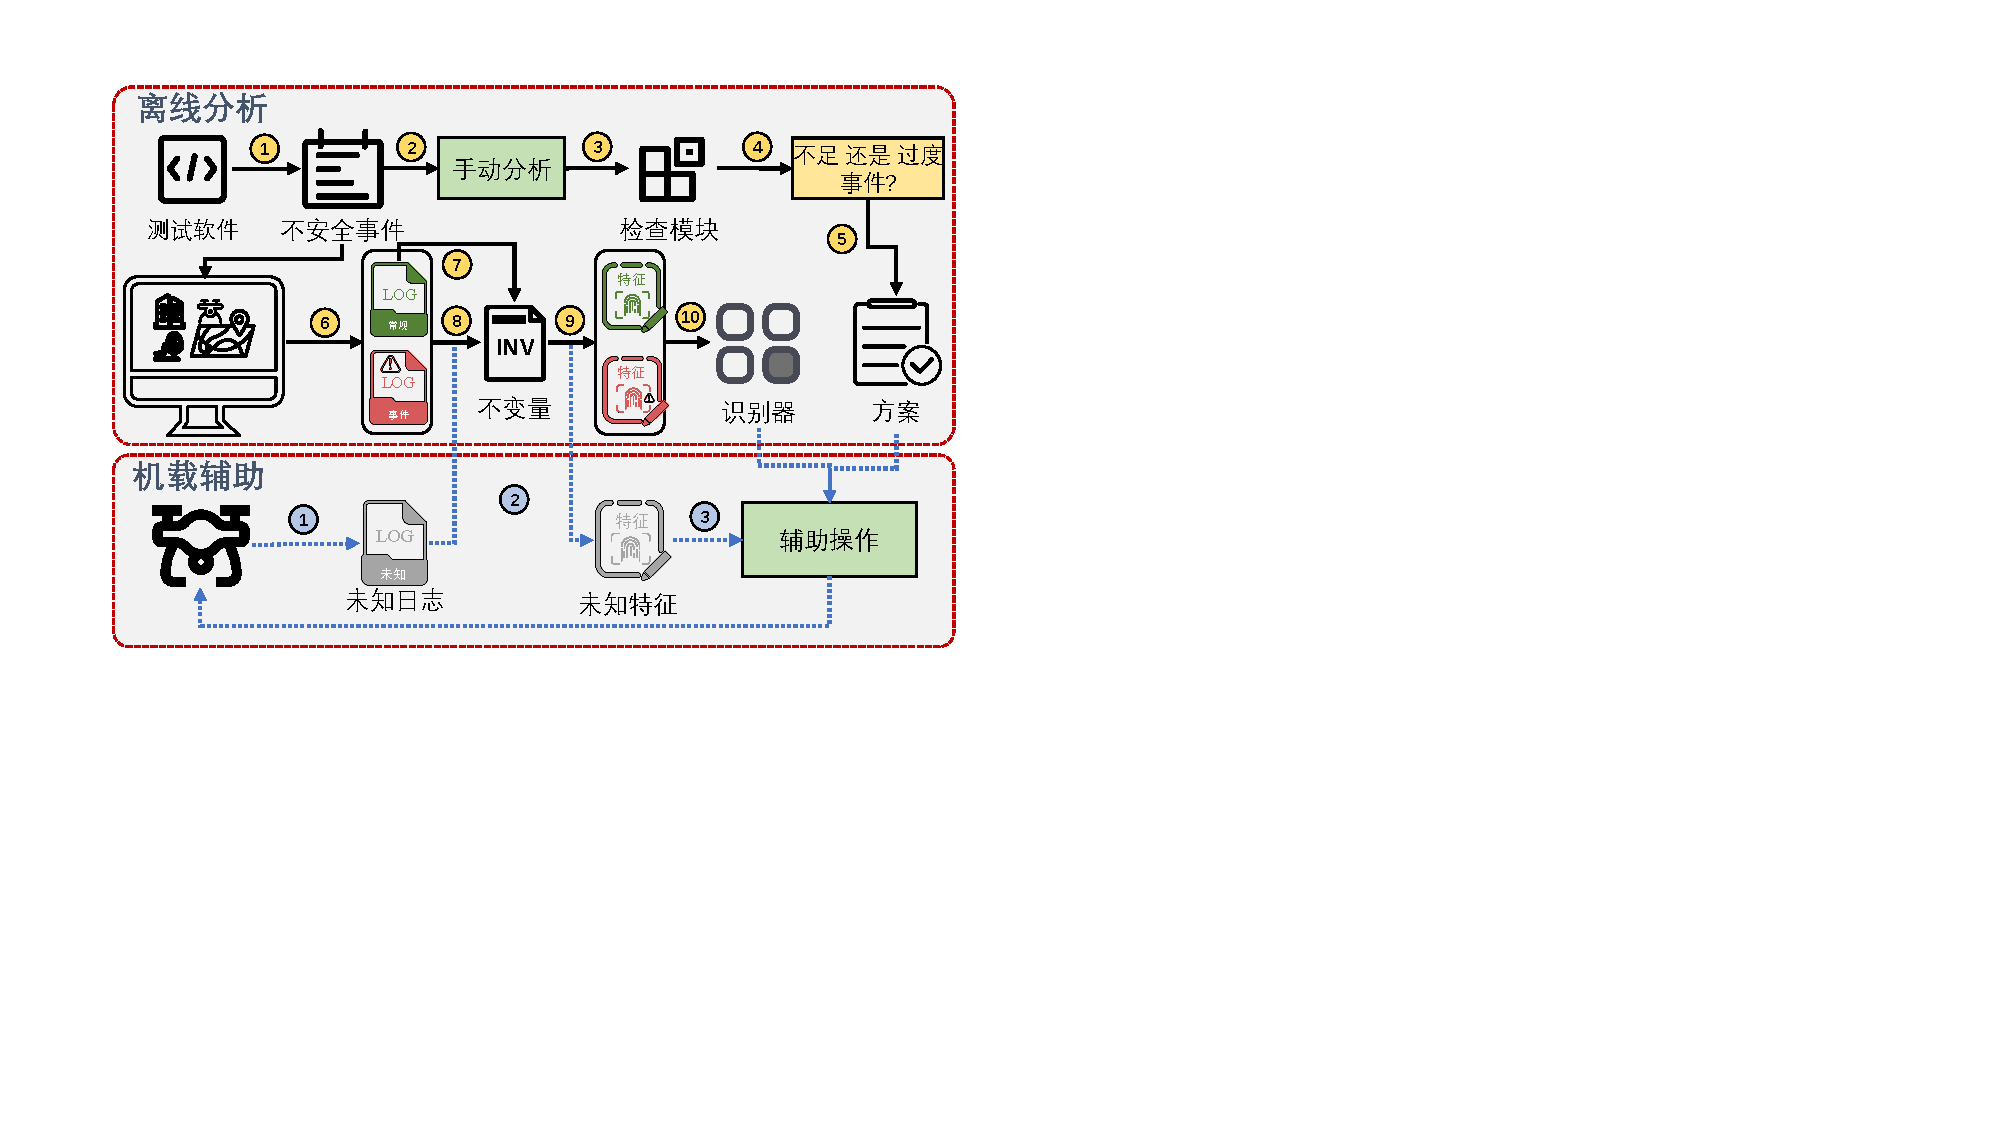
\includegraphics[width=\linewidth]{fig/check/overview_check.pdf}
\caption{\deccheck 流程和子模块}
\label{fig:check_overview} 
\end{figure}


\subsection{事件发现和分析}
\deccheck 首先应用模糊测试方法~\cite{choi2020cyber}来发现不安全事件。
对于不同类型的安全检查模块,\deccheck 使用不同的策略。
参考模块的官方文档或源代码,如果模块补救描述中包含控制操作或电力系统变化,则策略设置为搜索那些触发条件但不引起不稳定的事件(\emph{过度事件});如果模块补救只提出警告或简单的飞行模式切换,则策略设置为搜索那些引起不稳定但不触发条件的事件(\emph{不足事件})。
而根据它们的类别,\deccheck 采用不同的反应方案:(1)对于\emph{不足事件},\deccheck 为控制程序会发布一个新的警告,(2)对于\emph{过度事件},\deccheck 则中断它们的补救工作。


\subsection{数据收集}
由于不变量和检测器的生成需要数据训练,而无人机没有标准的数据集,所以实验手动发起数据采集,建立数据集。
而考虑到在不同的环境中很难提供真实的飞行,而且造成硬件损坏的概率很高,所以系统应用\tool{Airsim}模拟器~\cite{airsim2017fsr}来进行虚拟飞行实验。
\tool{Airsim}是一个真实的无人机飞行器模拟器,开发者可以获得内部飞行信息,包括飞行器的姿态、环境风速、碰撞信息和飞行日志。

\deccheck 进行两种实验来收集相应的数据--常规飞行和不安全事件。
常规飞行实验记录了没有任何物理事件影响的常规飞行状态数据。
不安全事件实验是针对不同场景下的每种不安全事件进行的。
每个飞行日志包含多个条目,由状态信息(如角度位置、加速度和油门速度)、传感器数据(如GPS、陀螺仪和加速度计)以及时间戳索引组成。
特别是,不安全事件日志只记录从事件开始到结束的时间戳。


\subsection{飞行状态不变量}
正如先前章节~\ref{moti:pre_study}中所介绍的有关无人机的飞行控制逻辑。
除非有干扰事件发生,控制算法的生成期望结果与实际的实现结果通常保持一个较小的偏差(甚至没有偏差)。
利用这一特性,\deccheck 建立一个状态不变量来模仿无人机状态估计逻辑。
在理想情况下(无干扰的常规飞行),实际状态将更接近于不变量预测的参考状态。
相反,如果实际的飞行状态与状态不变量给出的状态存在较大偏差,则认为当前状态偏离了不变量规定的飞行状态模式。
偏差值可以用来衡量当前状态的偏离程度。
以下通过\emph{飞行数据预处理}和\emph{状态不变量提取}两个小章节介绍如何处理数据以及生成不变量。

\subsubsection{飞行数据预处理}
所收集的飞行日志为一个列表,每个日志内都包含了飞行信息,如常规位置、陀螺仪传感器数据和时间戳。
但其中并不是所有的数据都对不安全事件的影响敏感。
考虑到不安全事件主要影响飞行姿态,系统采用了与姿态相关的状态和传感器数据:
(1)状态数据中的角位置和角速率,每一个都包含三个欧拉角,即Roll、Pitch和Yaw;
(2)从陀螺仪和加速度计获得的数据,每一个都包含沿X、Y和Z轴的三个数值。
同时,由于状态和传感器数据具有不同的更新频率,系统对具有高更新频率的数据进行采样,并使用时间戳作为索引,使其与具有较低更新频率的数据保持一致。
最终,时间戳$t$的数据向量形式为$v_t=\{a_t, e_t\}$,其中$a_i$和$e_i$是状态和传感器数据。
为了消除数据分布造成的不良影响,系统通过\tool{最小-最大尺度缩放}将特征值归一到$[0, 1]$之间。


\subsubsection{状态不变量提取}
由于物理世界中的不安全事件的飞行状态是复杂的、非线性的,在拟合模型中传统的线性拟合方法效果较差。
\deccheck 利用\tool{长短期记忆网络(Long Short Term Memory Networks,LSTM)}~\cite{hochreiter1997long}这种非线性学习模型方法来生成状态状态不变量,图~\ref{fig:check_invariant}总结了其原理和功能。
从功能上讲,状态不变量以$h$的连续向量$\{v_{t-h-1},...,v_{t-1},v_t\}$作为输入,并返回下一个时刻数据$v_{t+1}'$中的参考状态$a_{t+1}'$的最大条件概率预测值。

在训练阶段,模型通过最小化\tool{Mean Squared Error (MSE)}~\cite{4775883}来迭代更新其权重,从而减少预测的参考状态$a_{t+1}'$与地面真实状态$a_{t+1}$之间的偏差。
例如,假设一个样本数据是$\{v_1,v_2,v_3,v_4,v_5\}$。
如果设置窗口大小$h$=3,则该样本数据可以划分为输入和输出对$\{v_1,v_2,v_3; a_4\}$和$\{v_2,v_3,v_4; a_5\}$。
该模型通过学习$\{v_1,v_2,v_3\rightarrow a_4\}$的这种输入输出关系来更新其内部的网络模型权重,从而达到在输入为$\{v_2,v_3,v_4\}$时有最高的概率输出$a_5$。

\begin{figure}[ht]
  \centering
    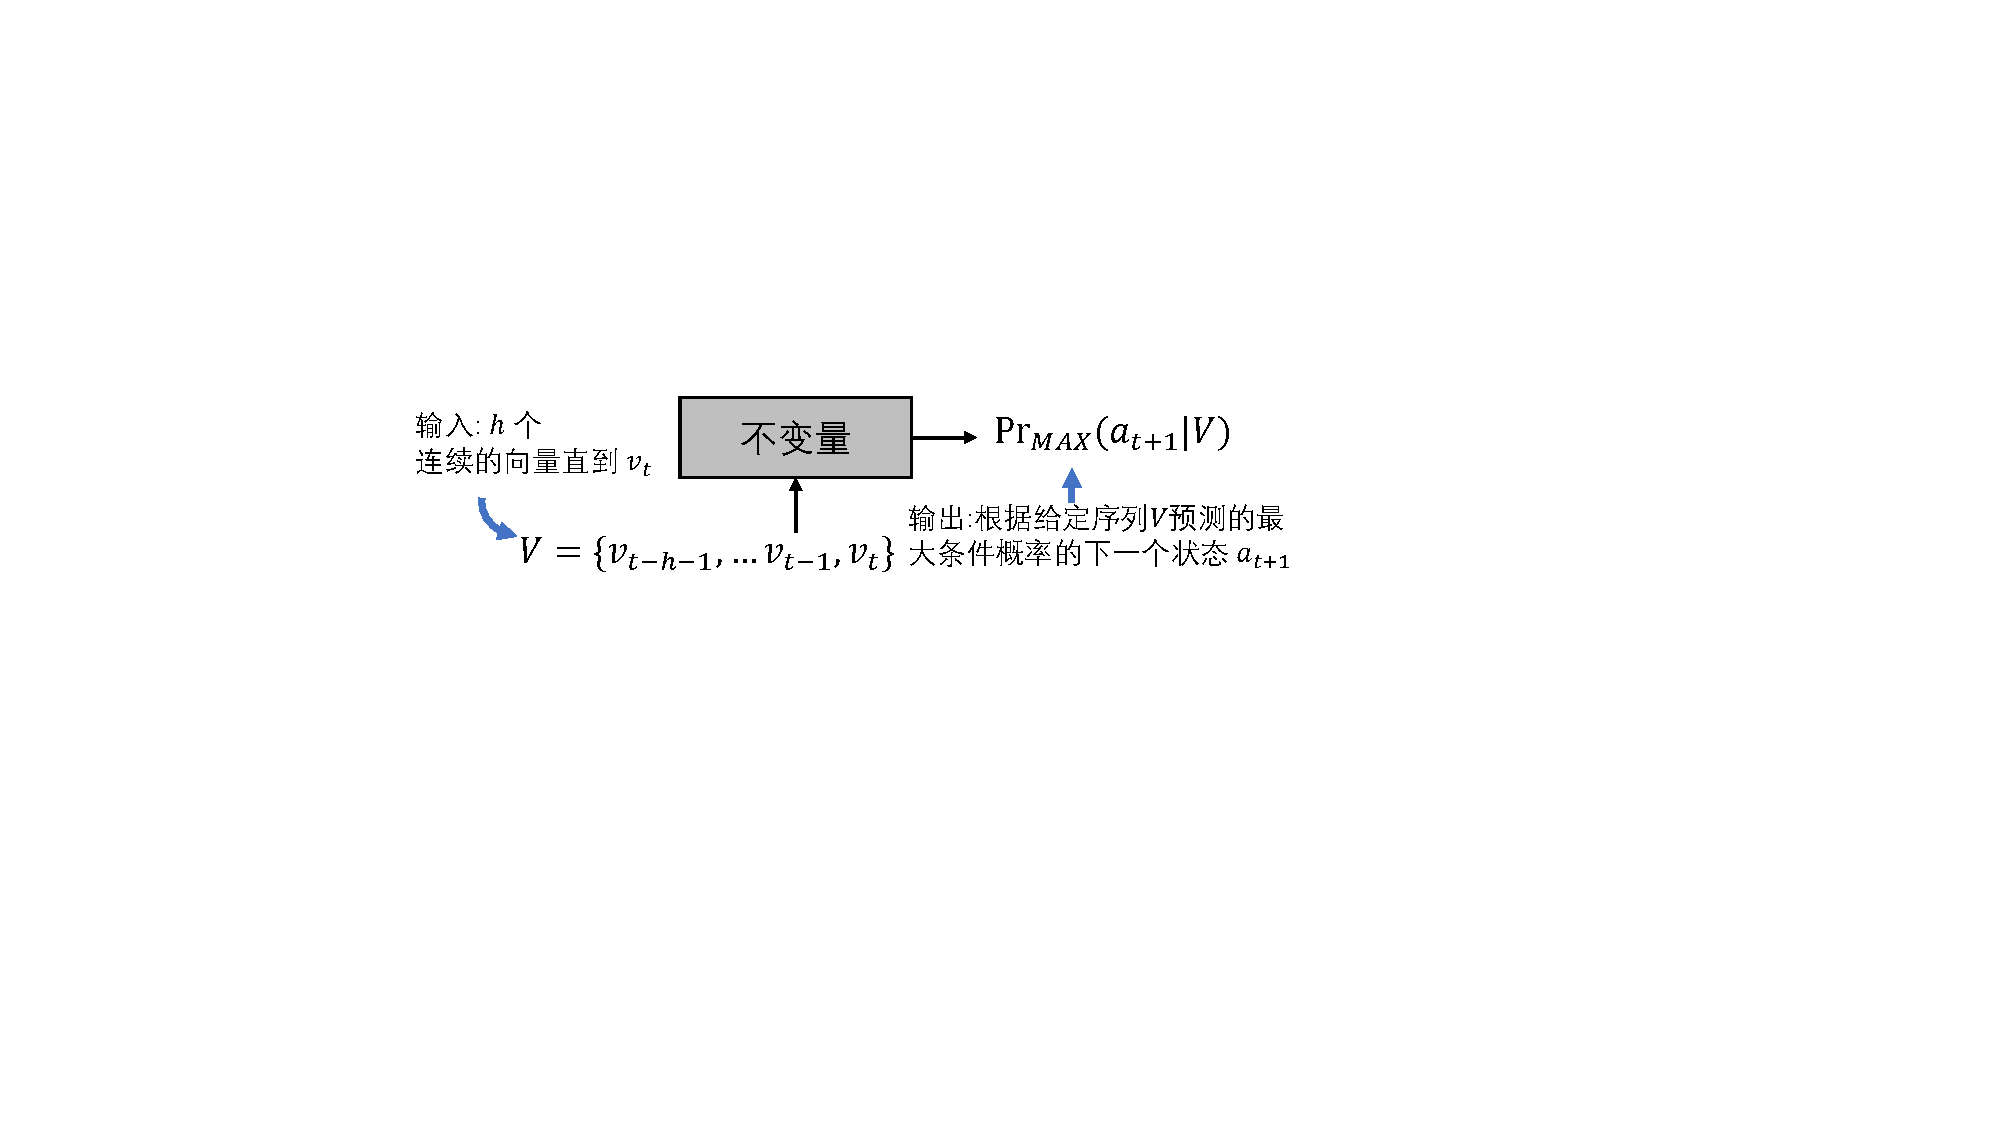
\includegraphics[width=\columnwidth]{fig/check/invairant.pdf}
\caption{飞行状态不变量的功能说明}
\label{fig:check_invariant} 
\end{figure}  

\subsection{不安全事件识别}
为了创建一个检测器来识别不安全事件,\deccheck 首先为每个不安全事件数据提取特征描述。
而为了确保同一类型的事件具有相同的特征模式,系统使用状态不变量来提取特征描述(称之为 \emph{段不变量偏差})。
该特征可以描述段中的异常数据,并保留系列值之间的关联性。
这种带有上下文相关属性的段特征可以减少单一异常数据的影响。
系统应用这些特征训练一个检测器来准确检测飞行中的这些不安全事件。
下文将详细描述从事件数据中提取特征、检测器训练和潜在不安全事件检测三个方面详解系统本身。

\subsubsection{特征描述提取}
给定一个事件数据,\deccheck 首先将其预处理为连续向量$V\{v_1,v_2,...,v_{n1}\}$,其中长度$n1$是事件的持续的时间戳长度。
由于事件有不同的持续时间(即长度$n1$),\deccheck 利用向量的滑动采样方法来生成具有相同形式的多个片段,其中长度与飞行状态包含元素个数的数量相同(在实现中长度为$6$)。
因此,一个事件数据可以产生多个片段$S_i$,规则如下。
\begin{equation}
S_i = \{v_i,v_{i+1},...,v_{i+5}\}, i\in[1,2,..., n-5]
\end{equation}
对于片段$S_i$,系统应用状态不变量来创建段预测$A'_i$,并计算它们之间的偏差称之为\emph{段不变量偏差}特征$SID$。

假设一个段为$S\{v_{1},v_{2},...,v_{6}\}$,下面将解释状态不变如何生成相应的预测段$A'$。
为了确保$S$能够生成相同大小的预测段$A'$,系统首先向$S$插入$h-1$行(与第一行的值相同),以获得填充段$S_{fill}$。
状态不变量使用这个填充段$S_{fill}$作为输入来生成预测状态段$A'\{a_1',a_2',...,a_6'\}$,规则如下。
\begin{equation}
a_j' = SI({v_j,v_{j+1},...,v_{j+h-1}}), j\in[1,2,...,6]
\end{equation}
其中$SI$是状态不变量,$v_j$是$S_{fill}$中索引为$j$的特征向量。
随后,系统选择$S$中的状态数据$A\{a_1,a_2,...,a_6\}$,计算与预测段$A'$的偏差,生成段不变差特征$SID = \Vert A - A' \Vert$。

\subsubsection{识别器训练}
训练之前首先要为事件提取的特征手动标记地标记标签。
考虑到$SID$是一个矩阵,先前的研究~\cite{girshick2015fast,shin2016deep}表明CNN~\cite{cnn}对矩阵形式的特征有更高的分类效率,因此\deccheck 利用CNN来创建检测器。
虽然CNN可以从原始数据中自动提取特征,但段不变差提取了更高层次的特征,考虑了状态变化的背景。
与\emph{段不变差}特征相结合,CNN有效地利用了矩阵值的位置关系,增强了检测器的有效性,消除了异常值分布的影响。

\subsection{潜在不安全事件识别}
当获得飞行状态不变量和检测器后,\deccheck 将被部署于无人机中用来监测飞行状态。
由于无人机硬件(如\tool{Pixhawk}~\cite{meier2011pixhawk}和\tool{TauLabs}~\cite{ebeid2018survey})通常使用STM32等性能较弱的芯片,\deccheck 采取异步检测,避免影响控制程序的运行。
它不断捕捉飞行状态和传感器数据的机载计算机来检测不安全事件。
每当它捕捉到六个信息条目时,它就会生成分段不变差特征,并应用检测器来识别当前的飞行状态。
根据检测到的类别,\deccheck 为控制程序提供补充建议。
(1)如果该类别属于\emph{不足事件},系统会发出警告并提供中断飞行的建议。
(2)如果该类别属于\emph{过度事件},并且安全检查触发了特定的检查模块,系统将清除警告并提供继续飞行的建议。

\section{实验结果及分析}
本章节的实验通过评估\deccheck 的有效性来进行说明。
主要讨论了以下几个研究问题:
\begin{itemize}
    \item \textbf{研究问题1 不变量有效性:} 不变量是否可以有效地预测飞行参考状态并适用于试不同飞行器模型和环境场景?
       
    \item \textbf{研究问题2 检测性有效性:} 检测器能否识别出不安全事件?
    
    \item \textbf{研究问题3 效率与对比研究:} 相较于传统工具\deccheck 的优势是什么?
    
    
\end{itemize}

\subsection{实验设定}
\begin{itemize}
\item \textbf{实验程序:} 
四个配备了ArduPilot(4.2.0)控制程序,其中一个是现实的\tool{Pixhawk}~\cite{meier2011pixhawk}飞行器,配备了Raspberry Pi 4B板载计算机,三个是虚拟飞行器,包括:\tool{Airsim},\tool{Morse}~\cite{echeverria2011modular},和\tool{Gazebo}~\cite{koenig2004design}。

\item \textbf{实验环境:}
所有的模拟实验和训练都在一台 AMD Ryzen 3970X、64GB内存、RTX 3090和Ubuntu 20.04的服务器上运行。
为了收集无人机的日志数据,\deccheck 使用了\tool{Pymavlink}与无人机进行数据传输,该插件允许开发者进行任务分配、运行时监控和参数检查。

\item \textbf{实验载具:}
为了测试该变量对不同飞行器的适应性,实验利用五种飞行器。%(如图~\ref{fig:check_pix}所示)。
四个配备了ArduPilot(4.0.3)控制程序,其中一个是真实的\tool{Pixhawk}~\cite{meier2011pixhawk}飞行器,配备了Raspberry Pi 4B板载计算机,三个是虚拟飞行器,包括:\tool{Airsim},\tool{Morse}~\cite{echeverria2011modular},和\tool{Gazebo}~\cite{koenig2004design}。
另一个是虚拟飞行器是\tool{Jmavsim},与上面的其他飞行器不同,它装载的是PX4控制程序~\cite{px4}。

\item \textbf{学习模型的架构:}
LSTM模型由一个LSTM单元、
 一个退火层(退火率为0.1)、
一个带有ReLU的激活层、
    和一个全连接的输出层构成。
CNN模型由两个卷积层组成,分别有9个$6\times6$和9个$3\times3$的卷积层、
    一个Flatten层,
    一个$256$维度的激活层,和一个全连接输出层。
\end{itemize}


\subsection{实验数据收集}
本次实验首先利用了模糊测试工具~\cite{choi2020cyber}并发现了两类不安全事件:\emph{轻微碰撞}(\emph{不足事件}),主要为侧面碰撞或弹跳的碰撞;\emph{阵风晃动}(\emph{过度事件}),由短暂的风导致的机身晃动。
因此,本实验后续需要对者两种类型的数据进行收集,也需要正常的飞行数据用于不变量的提取。

为了满足数据的多样性要求,本次收集实验在不同的情况下进行。
飞行数据是在六个不同的环境中产生的,图~\ref{fig:check_airsim}展示了其场景内容,皆由\tool{Airsim}工具发布,其中包含基本空间、足球场、废弃公园、室内场景、城市街区和有移动车辆的大型城市,每个模拟环境由各种物理组件组成。

\begin{figure}[htb]
\centering{
\subfloat[基本空间]{
\includegraphics[width=0.3\columnwidth]{fig/check/airsim/block.png}}\quad
\subfloat[足球场]{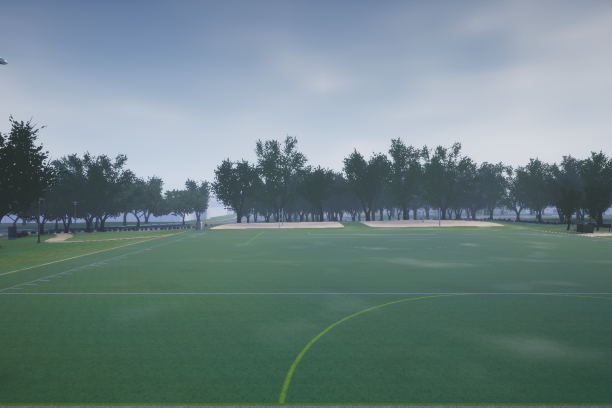
\includegraphics[width=0.3\columnwidth]{fig/check/airsim/ms.png}}\quad
\subfloat[废弃公园]{
\includegraphics[width=0.3\columnwidth]{fig/check/airsim/park.png}}
}
\centering{
\subfloat[室内场景]{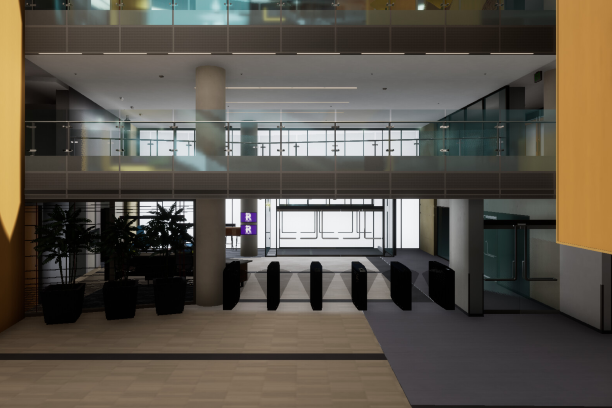
\includegraphics[width=0.3\columnwidth]{fig/check/airsim/building.png}}\quad
\subfloat[城市街区]{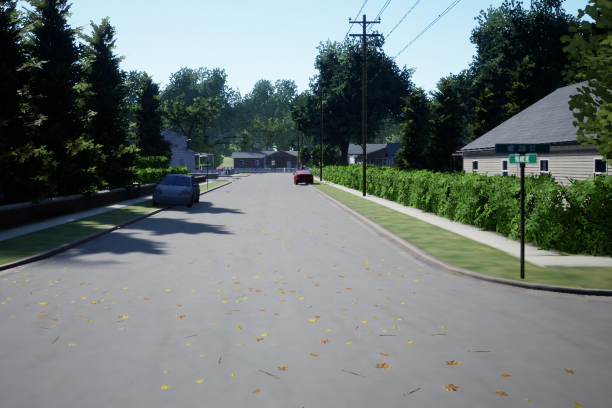
\includegraphics[width=0.3\columnwidth]{fig/check/airsim/neighborhood.png}}\quad
\subfloat[大型城市]{
\includegraphics[width=0.3\columnwidth]{fig/check/airsim/city.png}}
}

\caption{Airsim中不同场景的模拟环境}
\label{fig:check_airsim} 
\end{figure}

其中常规和\emph{阵风晃动}实验在基本空间中进行,而\emph{轻微碰撞}实验则在所有六个模拟器环境中进行。
在进行常规和阵风晃动的飞行任务时,任务规划如图~\ref{fig:check_mission1}所示 (实线是实现的轨迹,虚线是计划的轨迹)。
每次任务的构成有图中的$16$个航点以随机的方式进行连接。
参考优秀商业无人机\tool{MavicPro2}~\footnote{\url{https://www.dji.com/hk-en/mavic-2?site=brandsite&from=nav}}的抗风能力,该产品能够抵抗六级风($8.0m/s \sim 10.7m/s$)。
因此,本次实验的阵风速度被定义在$8.0m/s$到$10.7m/s$之间,并持续时间为$1\sim3$秒。
对于碰撞任务,实验在虚拟环境中选择有更多障碍物空间的核心区域,以确保碰撞事件必须发生。
而在飞行过程中,如果发生了碰撞,但在三秒内没有出现落地的情况,实验就将其视为\emph{轻微碰撞}。
图~\ref{fig:check_mission2} 展示了两个有碰撞的飞行任务的例子,其中灰色物体是障碍物,橙色点是计划的飞行航点,绿色点是飞行起飞点,虚线是飞行任务路径,实线是无人机实现的路径,红色圆圈是碰撞痕迹。

\begin{figure}[htb]
\centering{
\subfloat[常规和阵风任务]{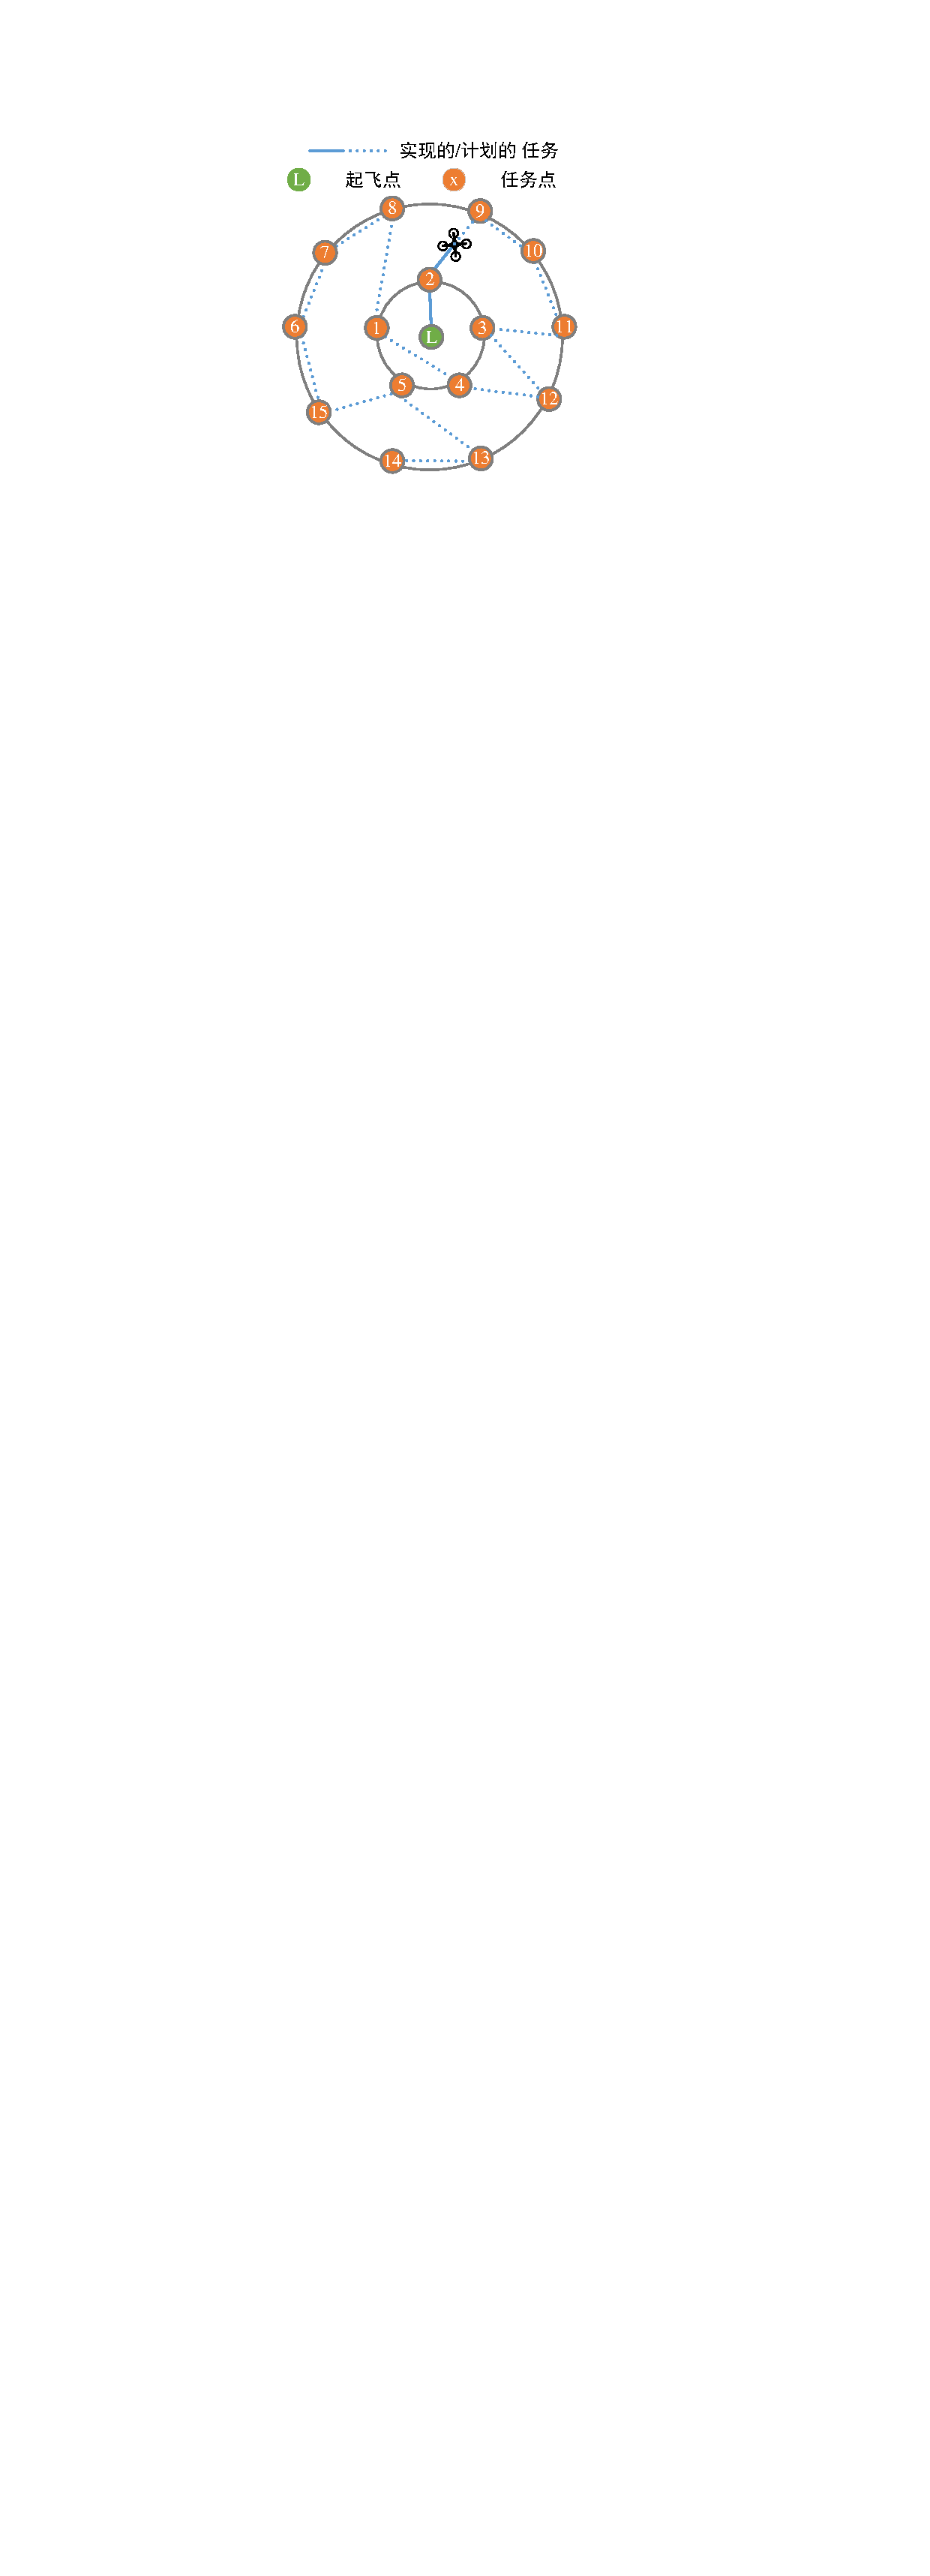
\includegraphics[width=0.35\columnwidth]{fig/check/ardupilot/mission.pdf}\label{fig:check_mission1} }
\subfloat[碰撞任务]{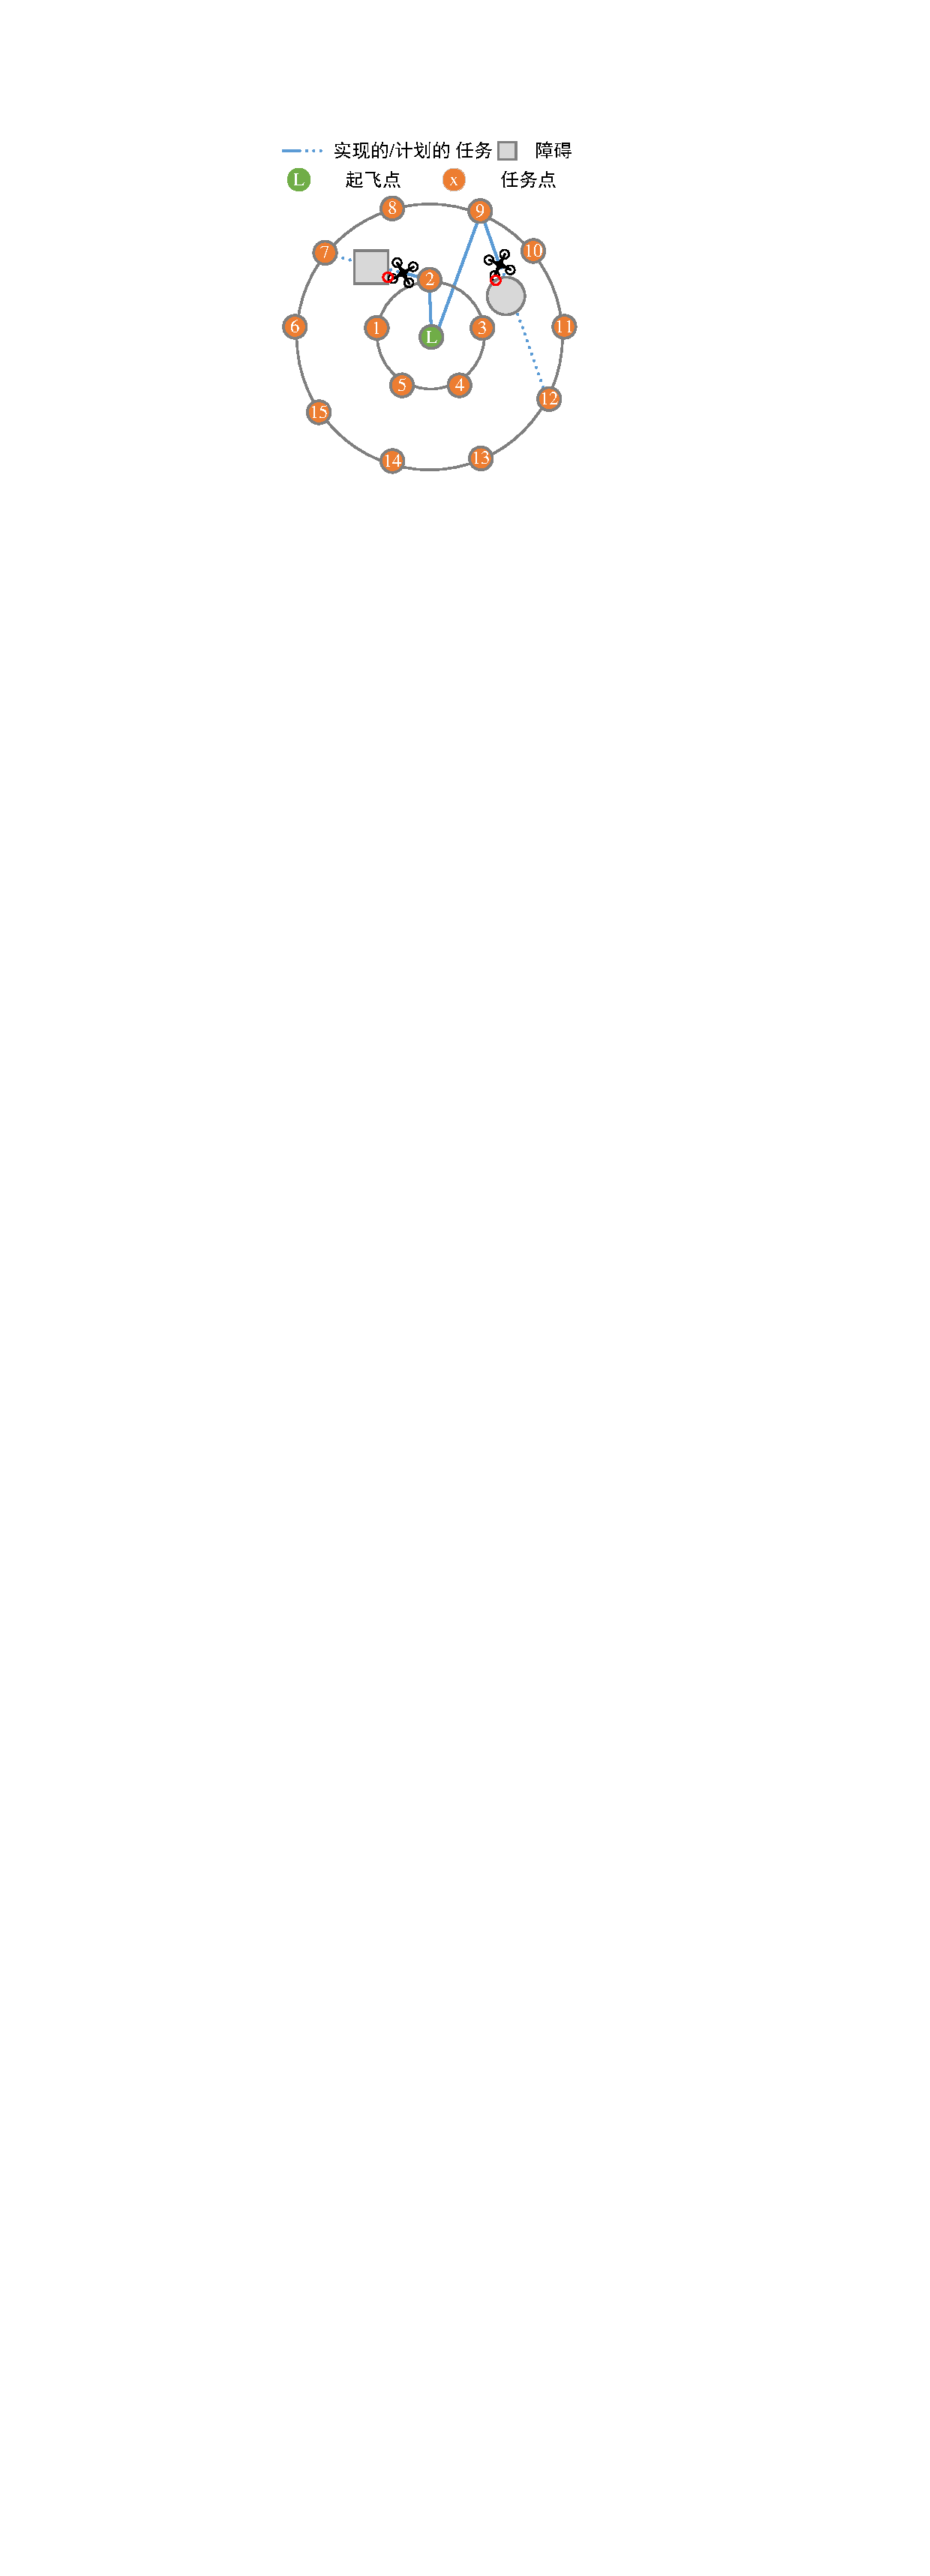
\includegraphics[width=0.35\columnwidth]{fig/check/ardupilot/mission2.pdf}\label{fig:check_mission2} }
}
\caption{飞行任务样例}
\label{fig:check_mission} 
\end{figure}

实验启动了$1,000$个常规飞行任务以产生飞行日志,并提取了$690,875$个飞行信息条目。
对于不安全事件检测的相关实验,实验启动了$1,000$个阵风实验,总共提取了$16,302$个信息条目;以及$1,000$个轻微碰撞实验,提取了$35,592$个信息条目。
为了进行比较,实验还选择了在章节~\ref{sec:check_problem}中描述的$100$个\emph{轻微碰撞}和$100$个\emph{阵风晃动}事件例子。


\subsection{提升评估标准}
由于系统的目标是处理\emph{不足事件}和避免由\emph{过度事件}引起的错误警报,安全检查的增强主要涉及两个指标,准确率(ACC)和假阳性率(FPR),定义如下。
\begin{equation}
    ACC = \frac{ TruePositive +  TrueNegative}{TotalPopulation}
\end{equation}

\begin{equation}
    FPR = \frac{FalsePositive}{ConditionNegative}
\end{equation}

其中$TruePositive$是正确识别的正例(即崩溃或推力损失)的数量。
    $TrueNegative$是正确识别的负例的数量。
    $TotalPopulation$是整个样本的数量。
    $FalsePositive$是被错误地标记为正例的样本数。
    $ConditionNegative$是被标记为负例的样本数量。
\deccheck 的目标是找到尽可能多的\emph{不足事件}(即增加ACC),并减少被错误地标记为正例的样本数量(即减少FPR)。


\subsection{研究问题1: 不变量有效性}
这个实验展示提取状态不变因素的过程,并验证了它可以有效地预测飞行状态的变化。
此外,本章节还评估了状态不变因素对环境风和飞行器模型的适应性。

\subsubsection{状态预测}
实验将$690,875$个收集到的数据分成$621,788$个用于训练状态不变量,剩下的$69,087$用于性能测试。
为了保证实验的真实性和可重复性,实验采用5折交叉验证法来记录不同输入$h$的平均准确率。
经过多轮的模型训练,不变量的预测性能如表~\ref{tab:check_cross}所示。
在不同的输入长度下,不变量的预测准确率都高于$98\%$,这说明不变量可以有效地预测参考状态,输入长度对预测的影响有限。
但为了得到最好的不变式以进一步建立特征,实验设定$h=2$,并选择性能最好的不变式模型进行后续实验。

\begin{table}[ht]
\caption{不同输入大小和测试数据集折叠的模型精度
}
\label{tab:check_cross}
\centering
\begin{tabular}{c|c|c|c|c|c|c}
        \toprule[1.5pt]
        输入长度  & 组1 & 组2 & 组3 & 组4 & 组5 & 平均 \\
      \midrule[0.8pt]
        1  & 0.9877 &	0.9877 &	0.9879 &	0.9881 &	0.9888 &	0.9880 \\
        
        2  & 0.9893 &	0.9903& 	0.9885 &	0.9914 &	0.9912& 	0.9901  \\
        
         3  & 0.9895 &	0.9898& 	0.9913 &	0.9904 &	0.9859 &	0.9894  \\
        
        4  & 0.9919 &	0.9874& 	0.9906& 	0.9916 &	0.9893 &	0.9901  \\
        
        5  & 0.9881 &	0.9901 &	0.9871 &	0.9892& 	0.9912 &	0.9891 \\
        \bottomrule[1.5pt]
\end{tabular}
\end{table}


\subsubsection{环境风适应性}
风是环境中最大的不确定因素。
实验进行了多次飞行任务以验证环境风是否影响了不变的预测。
实验分别发起$5$组飞行任务,每组包含$10$个飞行测试,每组的风速分别设置为$(0,1]$、$(1,2]$、$(2,3]$ 和 $(3,4]$ $m/s$。
测试将每组飞行实验的飞行数据条目输入到不变量当中来测试预测准确性,每组的平均结果如表~\ref{tab:check_wind}所示。
通过表可以观察到持续的风(不超过无人机性能的阈值)对不变预测的影响很小,平均准确度超过 $99\%$。
这是因为控制程序本身可以通过\tool{Kalman滤波}~\cite{vilez2015trajectory}来消除持续环境风的影响。
虽然一般的持续风对飞行影响不大,但是由于阵风震动具有持续时间短、风速大的特点,控制程序无法消除其影响,从而引发后续问题。
总体来讲,不变量模型不受持续正常风的影响,但可以有效地描述阵风的影响。

\begin{table}[ht]
\caption{不同风速下的模型精度}
\label{tab:check_wind}
\centering
\begin{tabular}{c|c|c|c|c}
        \toprule[1.5pt]
        风速级别(m/s) & \textbf{(0,1]} & \textbf{(1,2]} & \textbf{(2,3]} & \textbf{(3,4]}  \\
        \midrule[0.8pt]
        平均准确率  & 99.57\% & 99.49\% & 99.37\% & 99.17\% \\
        \bottomrule[1.5pt]
\end{tabular}
\end{table}

\subsubsection{飞行器适应性}
为了验证一个不变量是否具有普遍的适应性以应用到其他无人机飞行器模型上,测试实验使用不同的无人机设备测试状态不变量的预测准确性。
不变量从\tool{Airsim(ArduPilot)}无人机中提取,并将其应用于测试 \tool{Morse}、\tool{Gazebo}、真实无人机和 \tool{JMavsim} 的预测准确性。
具体方法为使用其他飞行器设备的飞行模型输入到不变量中来测试不变量的预测准确性。
表~\ref{tab:check_sim} 显示了不同车型的平均准确率。
从表中可以观察到,如果飞行器具有相同的控制程序(不论是模拟的还是现实的),状态不变量可以有效地预测它们状态的变化趋势,其准确度高于97\%。
但\tool{JMavsim (PX4)}这种具有飞行控制程序的表现结果较差。
这说明从某一特定飞行控制程序提取的不变量不适用于其他飞行控制程序,这是因为控制程序具有不同的状态估计逻辑和控制算法。
虽然如此,本方案依旧可以使用相同的流程来提取\tool{PX4}的状态不变量。


\begin{table}[ht]
\caption{不同车型的不变量预测准确性}
\label{tab:check_sim}
\centering
\begin{tabular}{c|c|c|c|c}
        \toprule[1.5pt]
        \multirow{2}{*}{车辆模型}&
        \multicolumn{3}{c|}{Ardupilot} & \multicolumn{1}{c}{PX4} \\
        
        \cmidrule[0.8pt]{2-5}
        
          & Gazebo & Morse & 真实无人机 & Jmavsim \\
        
         \midrule[0.8pt]
        
         准确率  & 97.30\% & 99.95\% & 99.87\% & 78.65\% \\
        
        \bottomrule[1.5pt]
\end{tabular}
\end{table}

\subsection{研究问题2: 检测性有效性}
此实验中主要验证了检测器的有效性,并选择了有代表性的样本来展示段不变差特征。

\subsubsection{有效性}  
实验首先使用状态不变量来生成不安全事件的特征,同时将特征作为数据集来训练检测器。
总体上讲,实验使用了$6,520$个常规飞行特征数据、$5,932$个\emph{轻微碰撞}特征数据、$2,717$个\emph{阵风晃动}特征数据,其中$5,868$常规飞行特征数据、$5,932$个\emph{轻微碰撞}特征数据、$2,717$个\emph{阵风晃动}特征数据用于训练分类器,其余的用于测试性能。
为了说明使用段不变差的必要性,作为比较,实验还训练了一个直接使用原始数据而不是段不变差特征的检测器。
两者都在测试数据中得到了验证,其性能如表~\ref{tab:cross_cnn}所示,其中\dquote{使用不变量}表示的是检测器应用段不变特征来训练的测试结果,而\dquote{不使用不变量}代表检测器直接使用原始段数据进行训练的结果。
从表中可以观察到,使用不变量的检测器具有更好的识别Precision,其F1-Score超过均$90\%$。
此外,与原始特征相比,使用不变量具有更平衡的Recall和F1-Score,也就是说,状态不变量对于复杂的不安全事件检测是有积极影响的。

\begin{table}[ht]
\caption{不同特征方式下物理安全事件检测的平均性能指标}
\label{tab:cross_cnn}
\centering
\begin{tabular}{c|c|ccc}
        \toprule[1.5pt]
        {特征} & {类别}  & {Precision} & {Recall} & {F1-Score}  \\
        \midrule[0.8pt]
        \multirow{3}{*}{使用不变量} & 轻微碰撞 & 98.20\% &   91.09\%  &  94.51\% \\
        
        & 正常飞行  & 92.02\%  &  99.58\%   & 95.65\% \\
        
        & 阵风晃动  & 97.38\%  &  86.67\% &   91.71\% \\
        \midrule[0.8pt]
        \multirow{3}{*}{不使用不变量} & 轻微碰撞 & 96.51\% &   92.48\%  &  94.45\% \\
        
        & 正常飞行  & 82.91\%  &  99.98\%   & 90.66\% \\
        
        & 阵风晃动  & 98.76\%  &  79.33\% &   87.99\% \\
        \bottomrule[1.5pt]
\end{tabular}
\end{table}

\subsubsection{不安全事件的特征案例}
本小节选择有代表性的事件数据样本段并展示使用不变量所生产的相应的特征。
图~\ref{fig:check_nnexample} 显示了\emph{轻微碰撞}和\emph{阵风晃动}的特征可视化值。
从图中可以清楚地观察到这两个事件样例都有清晰的异常值情况。
对于\emph{轻微碰撞}的例子,它标记了GPS故障、位置估计不良、故障安全和过度振动补偿激活的错误信息。
该事件影响了无人机的飞行状态,特别是Roll、Pitch和Pitch Rate。
至于\emph{阵风晃动}的例子,瞬时阵风会导致无人机向某个方向连续漂移,导致矩阵的某些列产生异常的持续。
两者之间的差异可以用分段不变的差异来清楚地描述。
图~\ref{fig:check_cov_kernal} 展示检测器识别这两个特征的热图,其中颜色深的部分表示这部分的数据在检测器识别中起到了较为主要的作用。
可以观察到,检测器的关注区域与实际产生差异的区域相近。


\begin{figure}[htb]
\centering{
\subfloat[
段不变差的示例,
颜色深浅表示原始值和预测值之间的偏差
]{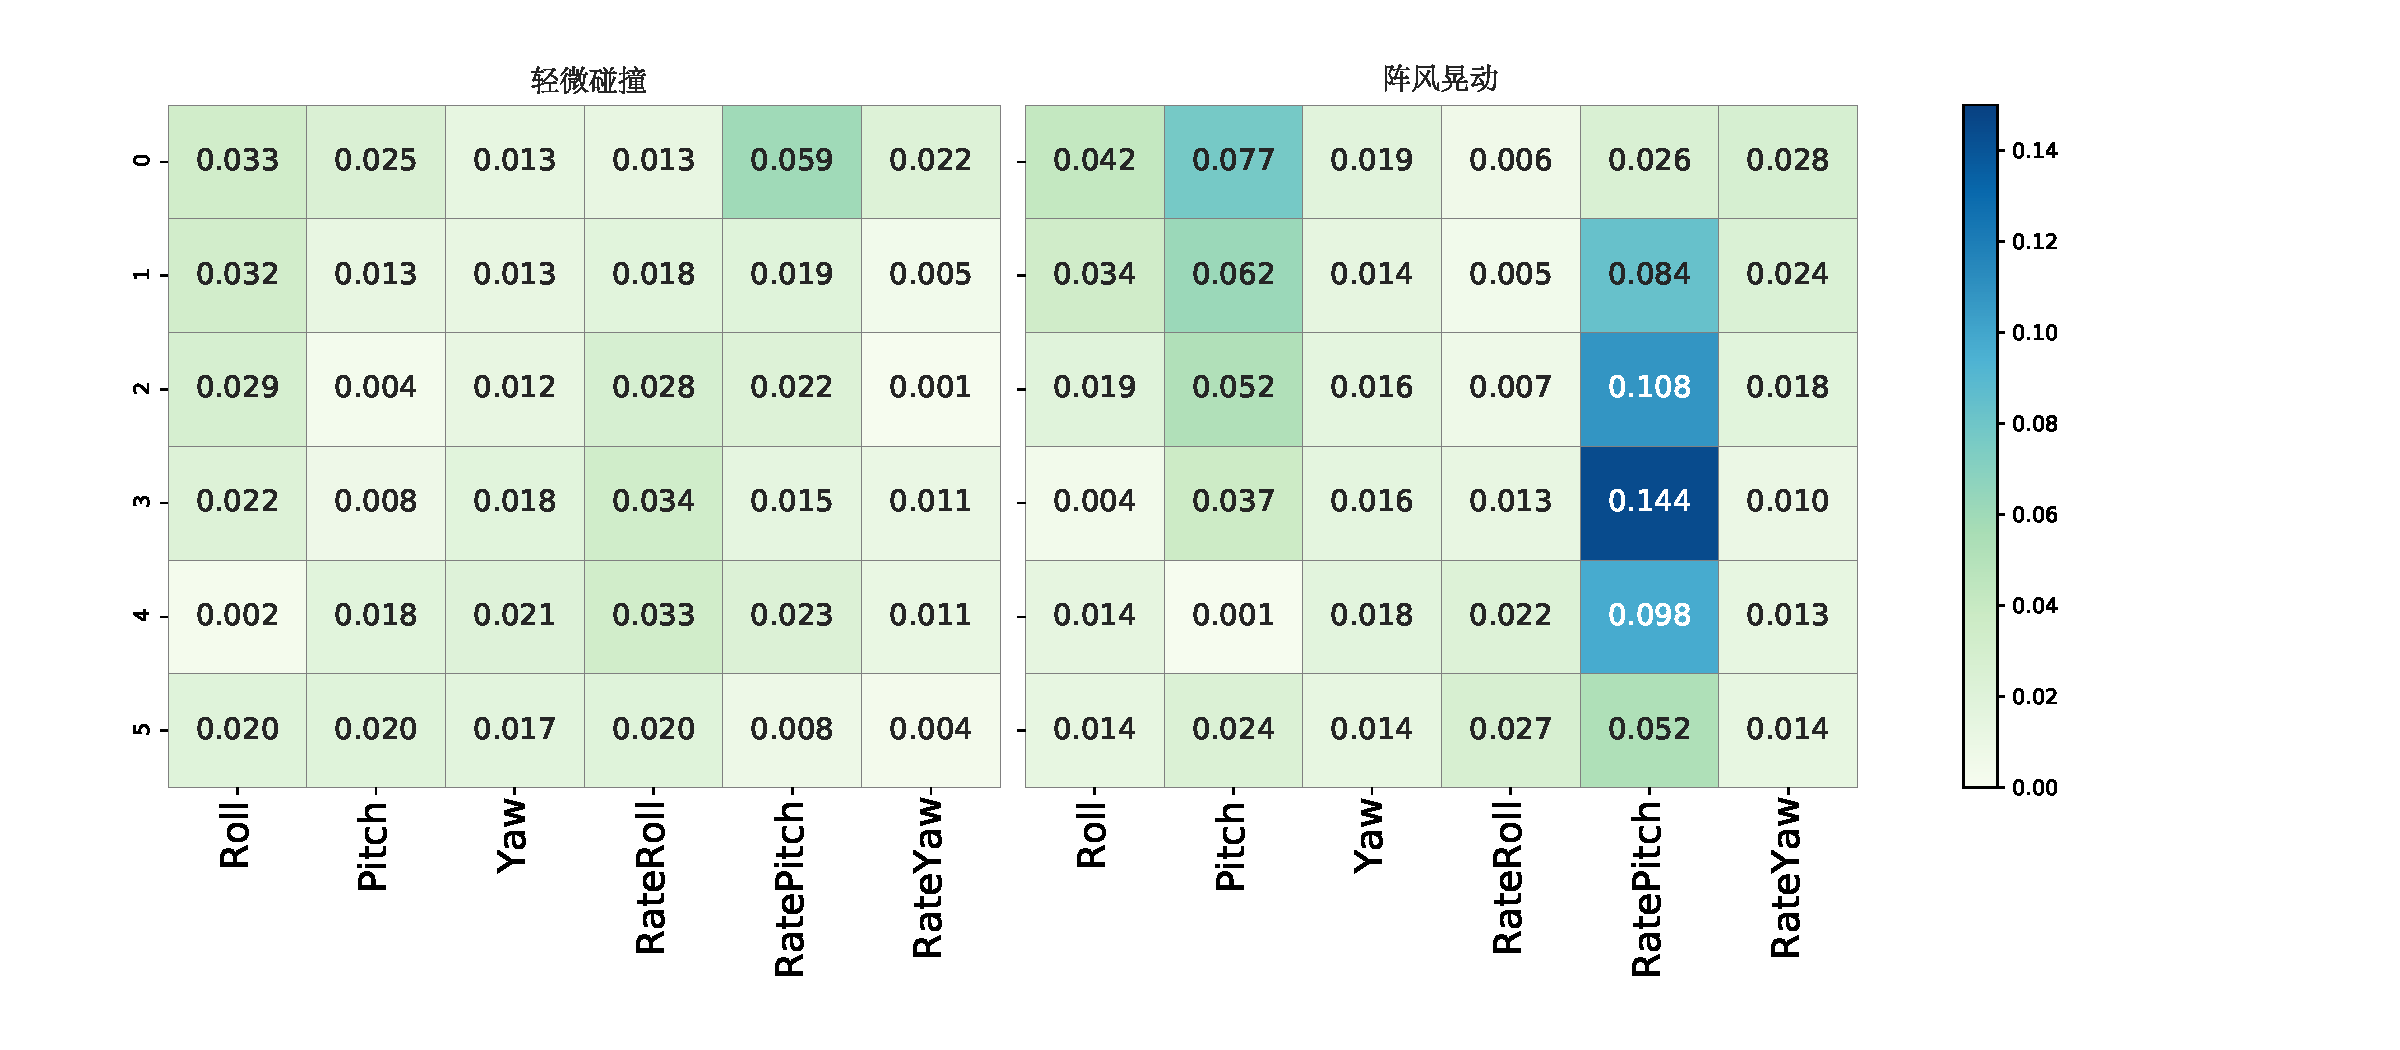
\includegraphics[width=\linewidth]{fig/check/nn/example.pdf}\label{fig:check_nnexample}}
\centering{
\subfloat[
检测器决策类别的热图,
颜色深浅表示分类的决策权重
]{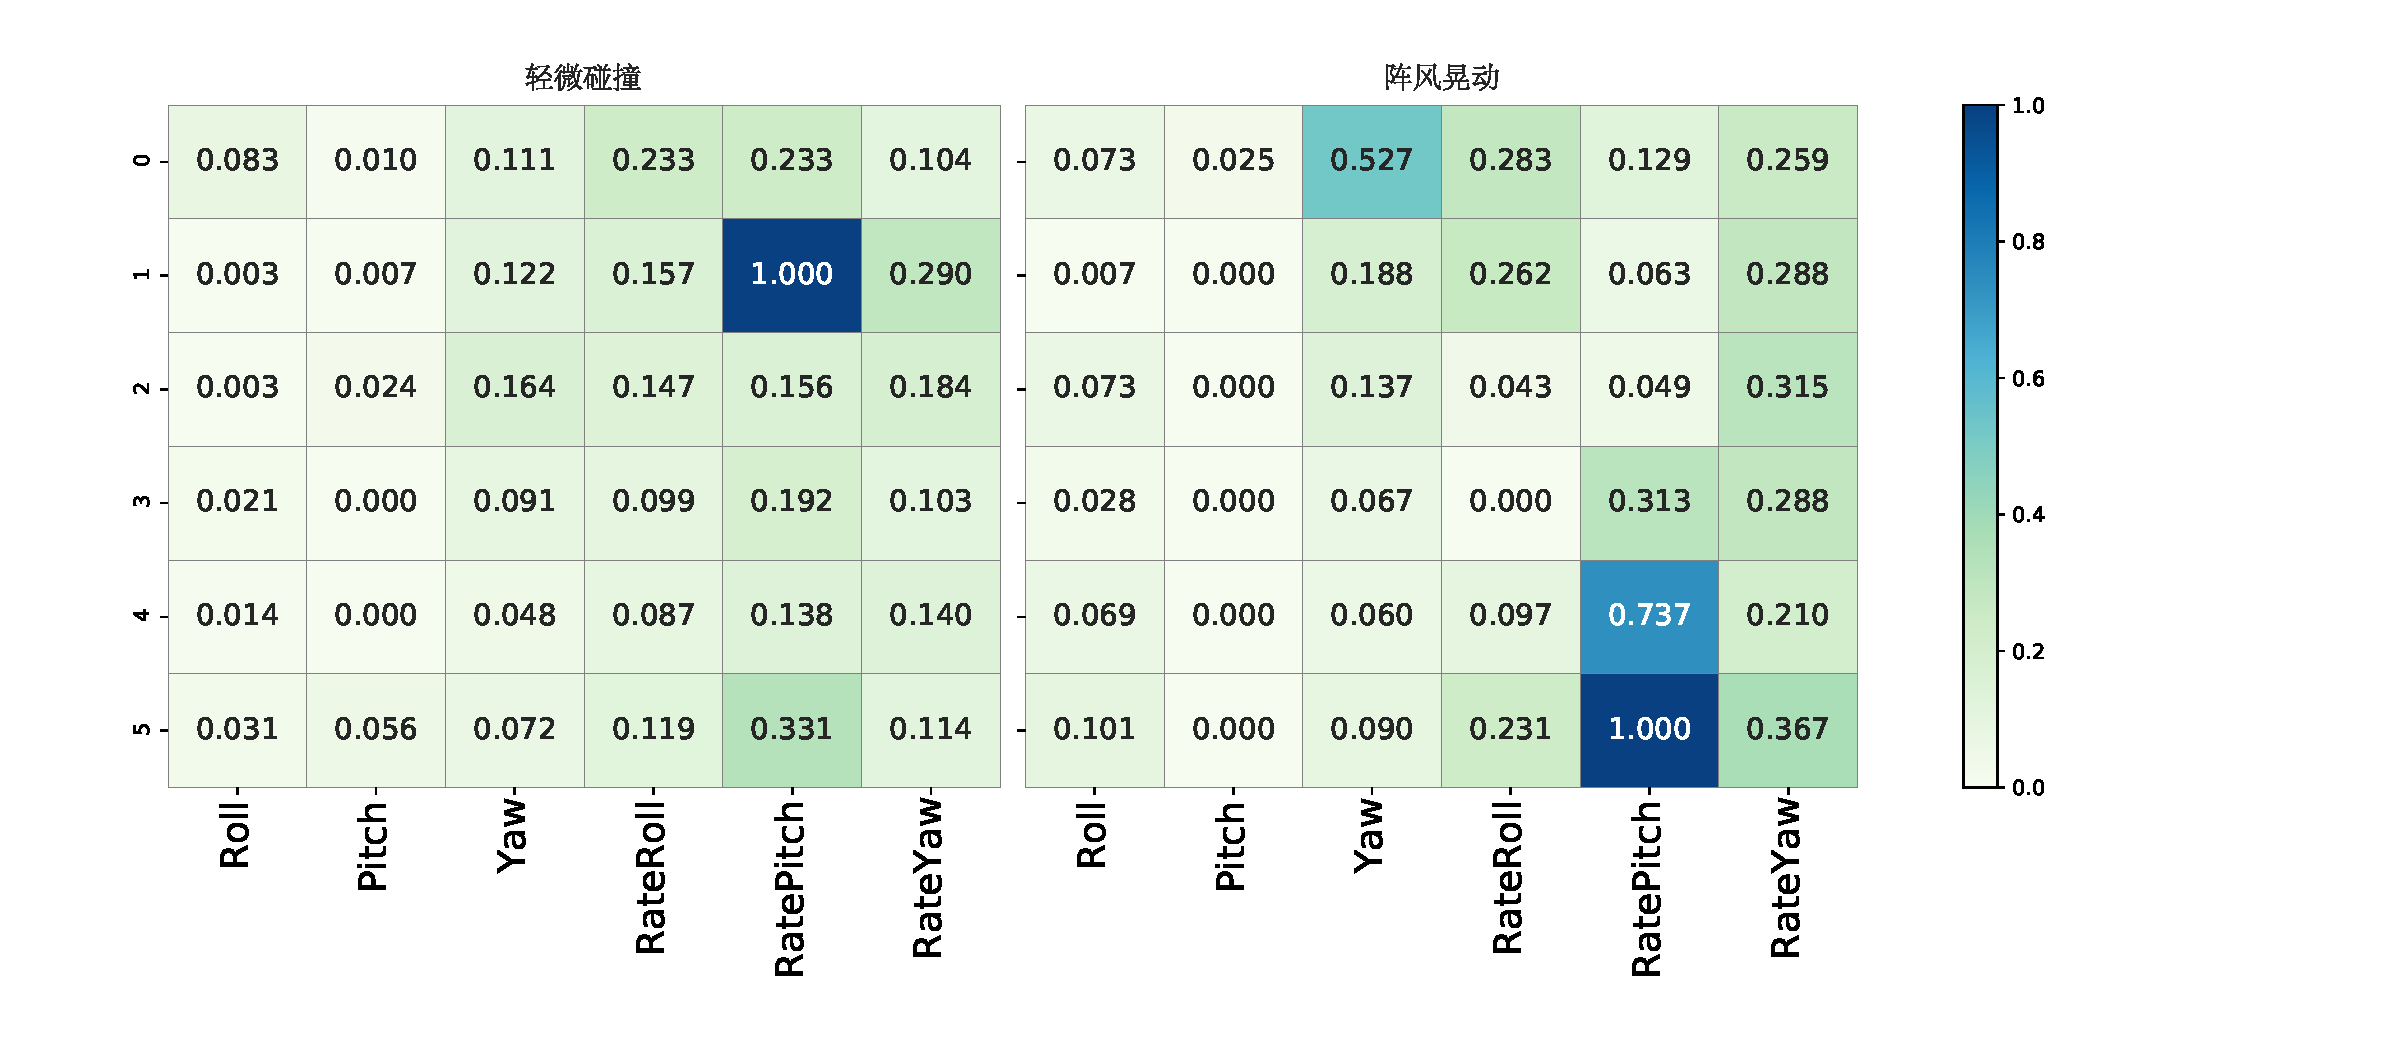
\includegraphics[width=\linewidth]{fig/check/nn/cov_example.pdf}\label{fig:check_cov_kernal}}
}
}
\caption{检测器决定热图样例} 
\end{figure}



\subsection{研究问题3: 效率与对比研究}
为了评估该系统是否能够提高处理复杂不安全事件的安全检查能力,此实验主要与原始安全检查系统进行了比较。
同时,为了显示其优势,本节实验还将其与其他较新的的异常检测方法进行了比较,这些方法包含\tool{SSR}~\cite{choi2020software}和\tool{PID-Piper}~\cite{piper}。
\tool{SSR}是一个用于飞行器的恢复框架,它通过线性模型预测来验证异常值并从不安全状态中恢复。
\tool{PID-Piper}是一个新颖的机器人飞行器的异常检测和飞行恢复系统,它应用非线性学习模型来实现与\tool{SSR}相同的功能。
需要注意的是,两者都有检测和恢复阶段,但在本实验只利用其异常检测阶段进行比较。

\subsubsection{功能提升}
实验使用与章节~\ref{sec:check_problem} 中一致的离线日志数据进行实验。
实验内容为使用\deccheck 去检查此前的飞行日志,看是否会触发其功能。
表~\ref{tab:check_cmp_check} 展示了\deccheck 的反应,其中\dquote{识别}表示\deccheck 识别的事件数,\dquote{辅助检查}代表安全检查的辅助修正。
原来的安全检查(见表~\ref{tab:check_crash_err})只识别出$2$个\emph{轻微碰撞},但实际上发生了$100$起\emph{轻微碰撞},而其汇报的$44$个推力损失信息均为误报。
与系统原始的安全检查相比,\deccheck 检测到 $81$\emph{轻微碰撞}和$76$\emph{阵风晃动}事件。
它补充了$79$ 碰撞警告并减少了$44$推力损失误报中的$36$个,这将碰撞检查的的ACC 从$2\%$ 增加到$81\%$,将推力损失检查的FPR 从$44\%$ 减少到$6\%$。

尽管\deccheck 可能会错误地检测到不安全事件(例如,将阵风震动报告为碰撞),但它不会对无人机造成致命后果,因为最终辅助判断是结合了原始安全检查和\deccheck 识别的。
由于安全检查没有推力损失警告,因此识别碰撞的假阵风震动检测不会生效。
至于识别阵风晃动时误判坠机,只会触发降落或返回操作,不会导致额外的威胁。

\begin{table}[ht]
\caption{\deccheck 对于安全检查的加强}
\label{tab:check_cmp_check}
\centering
\begin{tabular}{c|c|c|c}
        \toprule[1.5pt]
         {事件}  & {识别} & {辅助检查} & {修正} \\
         \midrule[0.8pt]
         轻微碰撞 & 81 & 碰撞检查 + 79  &  ACC: $2\% \to 81\%$\\
        阵风摇晃 & 76 & 动力损失误报 - 36 &  FPR : $44\% \to 6\% $ \\
        \bottomrule[1.5pt]
\end{tabular}
\end{table}
 

下面演示一个\deccheck 协助安全检查的例子。
实验进行了三个任务相同的飞行:常规飞行、阵风晃动飞行、阵风晃动但是装备了\deccheck 。
图~\ref{fig:check_pedec_work} 演示轨迹对比,其中红点为飞行轨迹点,白线为任务轨迹。
在常规飞行情况下(图~\ref{fig:check_dec_regular}),无人机可以右转并继续执行任务。
\emph{阵风晃动}事件会触发推力损失并启动电机助力,从而导致偏差(图~\ref{fig:check_dec_gust})。
在\deccheck 的帮助下,虽然安全检查发出了推力损失警告,\deccheck 确认这是\emph{阵风晃动}并中断了进一步的电机助力以保持正常飞行(图 ~\ref{fig:check_dec_pedec})。

\begin{figure}[htb]
\centering{
\subfloat[常规飞行]{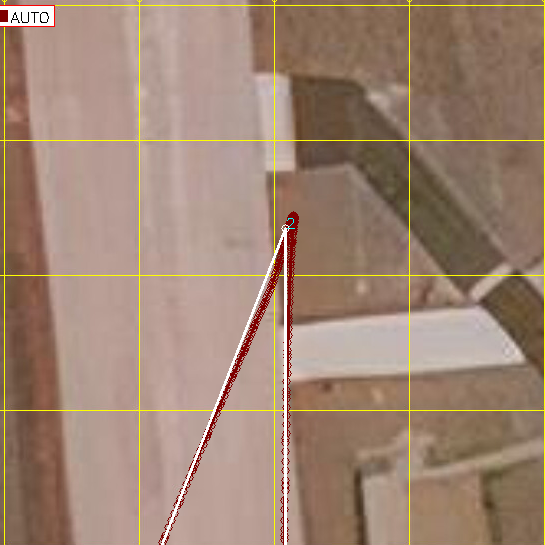
\includegraphics[width=0.32\columnwidth]{fig/check/cmp/regular.png}\label{fig:check_dec_regular} }
\subfloat[阵风晃动]{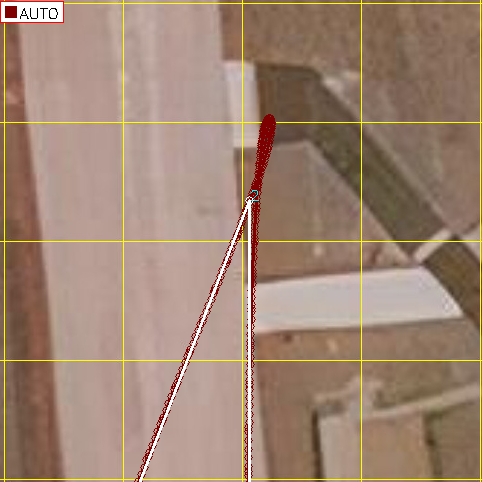
\includegraphics[width=0.32\columnwidth]{fig/check/cmp/gust.png}\label{fig:check_dec_gust} }
\subfloat[\deccheck]{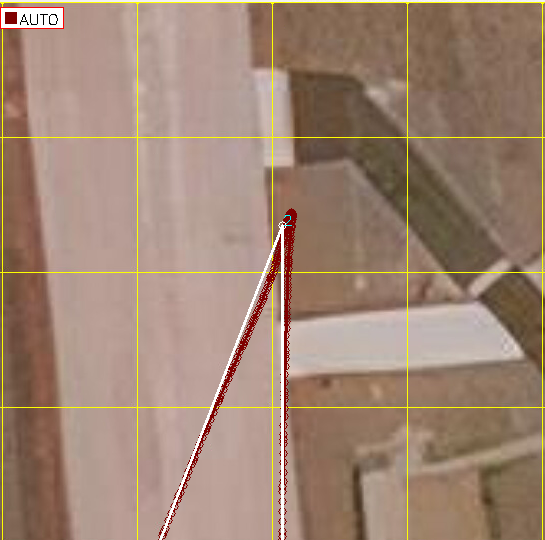
\includegraphics[width=0.32\columnwidth]{fig/check/cmp/pedec.png}\label{fig:check_dec_pedec} }
}
\caption{三种情况的飞行轨迹}
\label{fig:check_pedec_work} 
\end{figure}

\subsubsection{研究对比}  
对比研究使用相同的实验方法($100$ \emph{轻微碰撞}和 $100$ \emph{阵风晃动}事件)来展示三个系统的检测结果:\deccheck 、\tool{SSR} 和 \tool{PID-Piper}。
\deccheck 在不变量和检测器中使用最佳性能模型。
由于SSR不是公开可用的,此处实验使用其文章中公布的架构来实现相同的功能,识别但使用本实验相同的常规数据来进行训练。
对于 \tool{PID-Piper},参考源代码~\footnote{\url{https://github.com/DependableSystemsLab/pid-piper}}并使用本次实验的常规数据实现相同的架构模型。

\begin{figure}[ht]
  \centering
    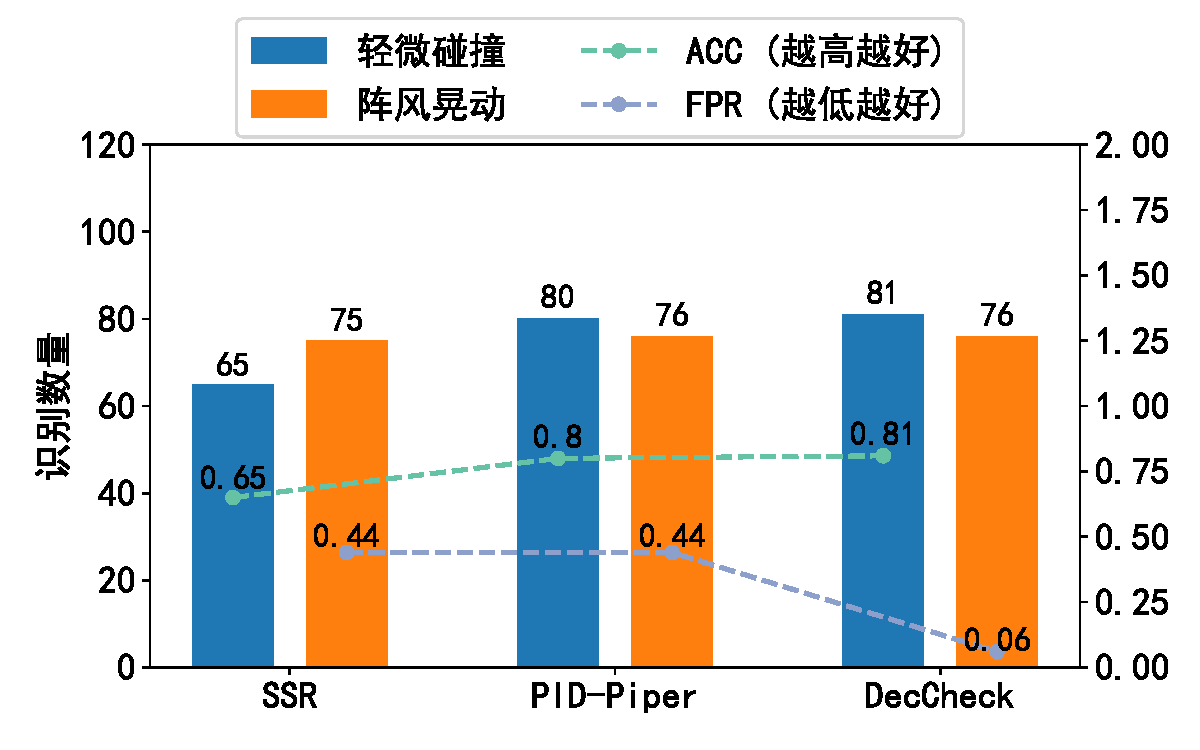
\includegraphics[width=\columnwidth]{fig/check/cmp/cmp.pdf}
\caption{\tool{SSR}、\tool{PID-Piper}和\deccheck 对物理事件的处理结果}
\label{fig:check_cmp} 
\end{figure}  

图~\ref{fig:check_cmp} 揭示了三个解决方案对于两种不同物理不安全事件的反应。
对于\tool{SSR} 和\tool{PID-Piper},他们分别检测到$65$个和$80$个\emph{轻微碰撞};
分别检测到$75$和$76$个\emph{阵风晃动}事件。
\deccheck 检测到 $81$ 个\emph{轻崩碰撞}和 $76$ 个\emph{阵风晃动}事件。
如果只评估异常检测结果,\deccheck 和 \tool{PID-Piper} 的性能优于最较早早提出的 \tool{SSR}。
因为无人机在其状态值之间具有非线性关系,因此线性方法 \tool{SSR} 可能会失去检测准确性。
但是如果考虑 ACC 和 FPR 的增强,\deccheck 具有最好的性能,它具有最高的 ACC,同时保持最小的 FPR。
这是因为 \tool{SSR} 和 \tool{PID-Piper} 只考虑异常检测而没有识别它们的类型。
它们采用相同的策略来处理不同的异常状态,这不适用于复杂的不安全事件。
虽然它们可以帮助系统安全检查增强\emph{轻微碰撞}检测的能力(提高 ACC),但它们不能降低推力损失的 FPR,这仍然会报告由\emph{阵风晃动}事件引起的异常反应。


\subsection{系统消耗}
在服务器训练阶段,LSTM需要$707.68$秒时间,CNN需要$23.87$秒的时间来优化学习模型直到达到收敛。
在检测阶段,根据飞行取样数据,Raspberry Pi 4B产生$10,000$的分段预测实例耗时$3.978$秒,验证$10,000$个的实例耗时$1.971$秒。
综上所述,机载计算机能够以合理的采样间隔有效地进行物理飞行事件的异步验证。

\section{本章小结}
本小节介绍了由于复杂的物理事件而导致的无人机安全检查系统出现错误反应的情况。
\emph{不足事件}不足事件会使得无人机安全检查系统无法正确的检出这类危险事件,从而导致系统错误判断自身问题并进一步造成安全问题。
\emph{过度事件}则是错误的引发了无人机安全检查系统的响应,但是这种错误的相应反而中断了无人机的正常飞行。
本小节通过\deccheck ,一个应用状态不变和机器学习检测器的系统来解决上述事件造成的问题。
\deccheck 建立的环境来收集各种事件数据,利用神经网络提取飞行状态不变量,最后应用不变量为每个事件创建相应的不变差异特征,并训练 CNN 模型来检测它们。
完备的实验证明也说明了\deccheck 系统在帮助无人机抵御这种复杂的事件上面有较大的提升。



